\documentclass[letterpaper,12pt]{article}

\usepackage{fullpage}
\usepackage{fancyhdr}
\usepackage[table]{xcolor}
\definecolor{highlight}{rgb}{0.46,0.98,0.59}
\usepackage{hyperref}
\definecolor{linkcolour}{rgb}{0,0.2,0.6}
\hypersetup{colorlinks,breaklinks,urlcolor=linkcolour, linkcolor=linkcolour}
%\hyperref[label_name]{''link text''}

\usepackage{array}
\usepackage{tabularx}
\usepackage[english]{babel}
\usepackage{multirow}
\usepackage{booktabs}
\usepackage{mathrsfs}
\usepackage{setspace}
\usepackage{lineno}
\usepackage{subfigure}
\usepackage{mathrsfs}
\usepackage{amsmath}
\usepackage{cite}
\usepackage{comment}
\usepackage{rotating}
\usepackage{array}
\usepackage{comment}
\usepackage{graphicx}

\usepackage{lmodern}
\usepackage[T1]{fontenc} 
\usepackage[latin1]{inputenc} 
\usepackage{textcomp}
\usepackage{lineno}

%for flowcharts
\usepackage{tikz}
\usetikzlibrary{shapes.geometric, arrows}
\tikzstyle{startstop} = [rectangle, rounded corners, minimum width=3cm, minimum height=1cm, text centered, draw=red]
\tikzstyle{io} = [rectangle, rounded corners, minimum width=3cm, minimum height=1cm, text centered, draw=black]
\tikzstyle{process} = [rectangle, rounded corners, minimum width=3cm, minimum height=1cm, text centered, draw=black]
\tikzstyle{decision} = [rectangle, rounded corners, minimum width=3cm, minimum height=1cm, text centered, draw=black]
\tikzstyle{arrow} = [thick, ->, >=stealth]

%for figures
\usepackage[export]{adjustbox}
\usepackage{wrapfig}
\usepackage[font=footnotesize,labelfont=it]{caption}

\usepackage{times}

\usepackage{url,parskip} 	%other packages for formatting
\usepackage{makecell}

\newcommand\sbullet[1][.5]{\mathbin{\vcenter{\hbox{\scalebox{#1}{$\bullet$}}}}}  %for bullet points inside table
\newcommand{\HRule}{\rule[20pt]{\linewidth}{0.3mm}}
\newcommand{\HRulesmall}{\rule[10pt]{0.5\linewidth}{0.3mm}}
\newcommand{\atlas}{{\sc Atlas}}
\newcommand{\cdf}{{\sc CDF}}
\newcommand{\TeV}{{Te\kern -0.1em V}}
\newcommand{\tev}{{Te\kern -0.1em V}}
\newcommand{\GeV}{{Ge\kern -0.1em V}}
\newcommand{\gev}{{Ge\kern -0.1em V}}
%\def\TeV{\ifmmode {\mathrm{\ Te\kern -0.1em V}}\else
%                   \textrm{Te\kern -0.1em V}\fi}%
\newcommand{\trileptoncdf}{\ensuremath{p\bar{p}\rightarrow \tilde{\chi}_2^0\tilde{\chi}_1^\pm \rightarrow \ell\ell\ell\nu\tilde{\chi}_1^0\tilde{\chi}_1^0  }}
\newcommand{\cnlep}{\ensuremath{\tilde{\chi}_2^0\tilde{\chi}_1^\pm \rightarrow \ell^+\ell^-\ell^\pm\nu\tilde{\chi}_1^0\tilde{\chi}_1^0}}
\newcommand{\dchlep}{\ensuremath{H^{++}H^{--}\rightarrow \ell^{+}\ell^{+}\ell^{-}\ell^{-} }}
\newcommand{\bprimelep}{\ensuremath{b'\bar{b}' \rightarrow WtWt \rightarrow WWbWWb}}
\def\ifb{\mbox{fb$^{-1}$ }}%  Inverse femtobarns.


\addtolength\topmargin{-1cm}
%\addtolength\oddsidemargin{-1cm}
%\addtolength\evensidemargin{-1cm}
%\addtolength\textwidth{2cm}
\addtolength\textheight{2.5cm}

%\setlength\oddsidemargin{1cm}
%\setlength\evensidemargin{1cm}

\newcounter{pubcount}

\include{definitions}

\begin{document}

%\linenumbers

%\pagestyle{empty} % non-numbered pages
\pagestyle{fancy}
\fancyhead{}
\fancyfoot{}
\renewcommand{\headrulewidth}{0.pt}
\renewcommand{\footrulewidth}{0.pt}
\fancyfoot[RO, RE] {\footnotesize{\thepage{} of }}
\fancyfoot[LO, LE] {\footnotesize{\it Srishti Patil - Project Report}}

\vspace*{2mm}

\thispagestyle{empty}
\begin{center}
\Large{\sc Signal Region Optimization for the search of Right Handed Neutrinos}
\end{center}
\vspace*{3mm}
\begin{tabular*}{\linewidth}{l@{\extracolsep{\fill}}r}
  \large{}& \large{Srishti Patil}\\
\end{tabular*}%
\vspace*{3mm}
\HRule
\vspace*{-2mm}

\section{Introduction}
\label{sec:intro}

The Standard Model of particle physics (SM) along with the theory of General Relativity (GR) can describe almost everything observed in nature, barring a few experimental and observational facts like baryon assymetry and the composition and origin of Dark Matter. \emph{Right handed neutrinos} (RHN), if they exist, could be responsible for a lot of these unexplained phenomena. They are promising Dark Matter candidates.

This project is a part of the search for RHN using data samples collected by the CMS experiment at the LHC in 2016 [Table~\ref{tab:samples}], corresponding to an integrated luminosity of 36 \ifb. We employ a technique called multilepton analysis [Section~\ref{sec:overview}]  for the search and the project focuses on a part of the process called Signal Region (SR) optimization [Section~\ref{sec:sro}]. The results obtained are used to produce limits on the production of right handed neutrinos.
\\

%feynman diagram
\begin{figure}[h!]
  \includegraphics[width=0.7\textwidth, center]{RHNfeynman.png}
  \caption{Illustrative leading order Feynman diagram for the production of RHN and its subsequent decay that may result in a multilepton final state. The taus can decay either hadronically or leptonically, giving us different channels to analyze that have different background profiles}
  \label{fig:rhnfeyn}
\end{figure}

\section{Overview}
\label{sec:overview}

The final state of an event (collision) is the set of particles seen by the detector. A lot of proceses Beyond the Standard Model (BSM) produce final states which majorly have multiple leptons, which is the motivation behind the development of a technique called Multilepton Analysis. Since a lot of SM processes also produce multilepton final states (called background), we use this strategy to distinguish signal from background.

The model considered here [Figure~\ref{fig:rhnfeyn}] includes a right handed neutrino ($N$) that decays into a \Wboson{} boson and a $\tau$, which decay further, giving rise to multilepton final states. For this analysis, we refer to electrons and muons collectively as light leptons ($\ell$). Events are then categorized by the multiplicity of light leptons and taus ($\tau$) in these final states, into the following channels: $3\ell$, $2\ell1\tau$, $1\ell2\tau$ and $3\tau$.

To begin with, we generate the RHN acceptance cutflow table [Section~\ref{sec:cutflow}, Table~\ref{tab:cutflow}] for both the tau IDs, to understand the process and how various triggers and selections affect the acceptance. Next, we attempt to understand the process of RHN production and decay at the gen-level [```ref section```] (\ie{} from simulations). Guided by the conclucions drawn from the study of these gen-level plots, we try to carve out a Signal Region [Section~\ref{sec:sro}] from the phase space which will give us good signal sensitivity. We use signal significance [```ref table```] as a metric to compare signal regions.   

%samples
\setcounter{table}{0}
\begin{table}[t!]
  \renewcommand\thetable{1}
  \centering
  \setlength{\tabcolsep}{30pt}
  \renewcommand{\arraystretch}{2}
  \resizebox{\textwidth}{!}{%
    \begin{tabular}{c|c|c|c}
      \hline \hline
        
      \multirow{2}{*}{\textbf{Sample (Mass Point)}} & \multirow{2}{*}{\textbf{Total Number of Events (n)}} &
      \multirow{2}{*}{\makecell{$\textbf{Cross-Section (xsec)}$\\
        $\textbf{(pb)}$}} &
      \multirow{2}{*}{\makecell{$\textbf{Luminosity}$\\
        $\textbf{(\ifb)}$}}\\
       & & & \\
      \hline
      \rule{0pt}{7ex}    
      100 $\GeV$ & 299,200 & 0.830 & 360.482 \\
      150 $\GeV$ & 286,200 & 0.119 & 2405.042 \\
      400 $\GeV$ & 200,000 & 0.00272 & 73529.411 \\
       & & & \\    
      \hline \hline
      
    \end{tabular}%
  }
  \caption{Data samples used for this analysis. Three mass points are considered and their respective sample luminosities are calculated using the formula $L_{sample}$ = n$_{sample}$ / xsec$_{sample}$}
  \label{tab:samples}
\end{table}

\section{Object and Event Selections}
\label{sec:selections}

To better identify particles significant to our analysis, we apply certain basic preselctions and triggers to the data. Object selections are listed in Table~\ref{tab:objselemu} and Table~\ref{tab:objseltau}. Triggers are listed below. In addition to these, a few corrections like MET filters (on data and MC both), tau energy scale corrections and tau reco scale factors are also applied.
\\

Triggers:
\begin{itemize}
\item Leading muon $\pt>26(29) \GeV$ for $2016$ \& $2018(2017)$
\item Leading electron $\pt>30(35) \GeV$ for $2016(2017$ \& $2018)$
\item For Single Muon PD, HLT\_IsoMu24 \& HLT\_IsoTkMu24 (in data only)
\item For Single Electron PD, HLT\_Ele27\_WPTight\_Gsf (in data only)
\end{itemize}

%object sel - e/mu
\begin{table}[h!]
  \centering
  \scriptsize
  \setlength{\tabcolsep}{30pt}
  \renewcommand{\arraystretch}{2}
  \resizebox{\textwidth}{!}{%
    \begin{tabular}{c|c}
      \hline \hline
      \makecell[c]{\textbf{Muons}} & \makecell[c]{\textbf{Electrons}}\\
      \hline
       
      \makecell[l]{\\$\sbullet \hspace{0.3cm} \pt>10, |\eta|<2.4$ \\
        $\sbullet \hspace{0.2cm}$ Prompt ($d_{xy}<0.05, d_{z}<0.1$ cuts)\\
        $\sbullet \hspace{0.2cm}$ POG Medium ID\\
        $\sbullet \hspace{0.2cm}$ Relative dB-corrected isolation \\$\hspace{0.3cm}$ tight WP $(<0.15$ in $\DeltaR=0.4)$}&
      
      \makecell[l]{\\$\sbullet \hspace{0.2cm} \pt>10, |\eta|<2.5$ \\
        $\sbullet \hspace{0.2cm}$Prompt ($d_{xy}<0.05(0.1), d_{z}<0.1(0.2)$ \\ $\hspace{0.3cm}$in barrel(endcap) region)\\
        $\sbullet \hspace{0.2cm}$Cut-based Medium ID\\
        $\sbullet \hspace{0.2cm}$Relative rho-corrected isolation \\$\hspace{0.2cm}$ Medium WP (included in ID)}
      \\
      \\
      \hline \hline

    \end{tabular}%
  }
  \caption{Object selections for light leptons}
  \label{tab:objselemu}
\end{table}

%object sel - tau
\begin{table}
  \centering
  \setlength{\tabcolsep}{30pt}
  \renewcommand{\arraystretch}{2}
  \resizebox{\textwidth}{!}{%
    \begin{tabular}{c|c}
      \hline \hline
      \multicolumn{2}{c}{\textbf{Taus}}\\
      \hline
      MVA ID (old) & Deep ID (new)\\
      \hline
 
      \makecell[l]{\\$\sbullet \hspace{0.3cm} \pT>20, |\eta|<2.3$ \\
        $\sbullet \hspace{0.2cm}$ Prompt ($d_{z}<0.2$ cut)\\
        $\sbullet \hspace{0.2cm}$ Old decayModeFinding, 1-prong \& 3-prong\\
        $\sbullet \hspace{0.2cm}$ '2017v2' ID\\
        $\sbullet \hspace{0.2cm}$ againstElectron \& againstMuon discriminators, loose WP\\
        $\sbullet \hspace{0.2cm}$ Cleaning against tight ID light leptons ($\DeltaR>0.4$)}  &
      
      \makecell[l]{\\$\sbullet \hspace{0.3cm} \pT>20, |\eta|<2.3$ \\
        $\sbullet \hspace{0.2cm}$ Prompt ($d_{z}<0.2$ cut)\\
        $\sbullet \hspace{0.2cm}$ New decayModeFinding, 1-prong \& 3-prong\\
        $\sbullet \hspace{0.2cm}$ Tau\_idDeepTau2017v2p1VSe $\geq 15$ \& \\ $\hspace{0.3cm}$ Tau\_idDeepTau2017v2p1VSmu $\geq 3$ (Loose WP)\\
        $\sbullet \hspace{0.2cm}$ Tau\_idDeepTau2017v2p1VSjet > 31 (Tight WP)}
      \\
      \\
      \hline \hline
      
      
    \end{tabular}%
  }
  \caption{Object selections for taus. A comparision between the two object IDs is given in Section~\ref{sec:cutflow}.}
  \label{tab:objseltau}
\end{table}
  
%event selection flow
\begin{wrapfigure}{r}{0.15\textwidth}
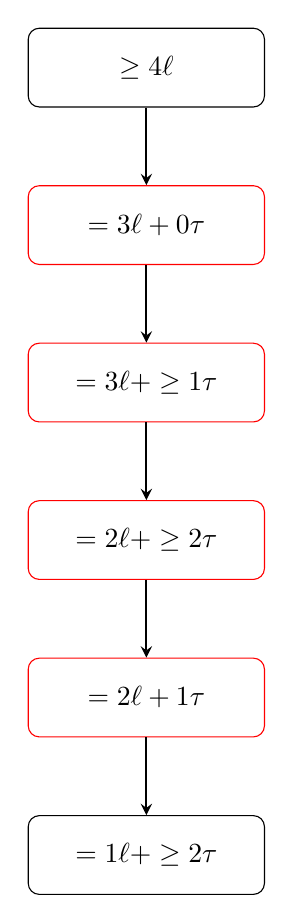
\begin{tikzpicture}[node distance = 2cm]
  \node(a)[io]{$\geq4\ell$};
  \node(b)[startstop, below of=a]{$=3\ell + 0\tau$};
  \node(c)[startstop, below of=b]{$=3\ell + \geq1\tau$};
  \node(d)[startstop, below of=c]{$=2\ell + \geq2\tau$};
  \node(e)[startstop, below of=d]{$=2\ell + 1\tau$};
  \node(f)[io, below of=e]{$=1\ell + \geq2\tau$};
  \draw[arrow] (a)--(b);
  \draw[arrow] (b)--(c);
  \draw[arrow] (c)--(d);
  \draw[arrow] (d)--(e);
  \draw[arrow] (e)--(f);
\end{tikzpicture}
\caption{Event selection flow}
\label{fig:eventselflow}
\end{wrapfigure}

The events used for analysis are selected only if they pass certain conditions. These selections are listed in Table~\ref{tab:eventsel}. An event is selected for a channel only if it fails the selections for all the previous channels. The order of priority (event selection flow) is illustrated in Figure~\ref{fig:eventselflow}. This project focuses on the 2$\ell$1$\tau$ and 3$\ell$ channels. The relevant states have been highlighted in red.

%event sel
\begin{table}
  \centering
  \setlength{\tabcolsep}{30pt}
  \renewcommand{\arraystretch}{1.2}
  \resizebox{\textwidth}{!}{%
  \begin{tabular}{l}
    \hline \hline
    \centerline{\textbf{Event Selections}}\\
    \hline
    \centerline{$3\ell$}\\
    \hline
    $\sbullet \hspace{0.2cm}$ Leading light lepton ($e/\mu$) passing triggers\\
    $\sbullet \hspace{0.2cm}$ Altleast two more light leptons ($e/\mu$), $\pt>10,10 \GeV$\\
    $\sbullet \hspace{0.2cm} \DeltaR>0.4$ among the three leptons\\
    $\sbullet \hspace{0.2cm}$ Minimum invariant mass of same flavor (SF) light lepton pair $> 12 \GeV$\\
    $\sbullet \hspace{0.2cm}$ Minimum $\DeltaR$ between all leptons in the event $> 0.4$\\
    $\sbullet \hspace{0.2cm}$ Triggers (in data only)\\
    \hline
    \centerline{$2\ell1\tau$}\\
    \hline
    $\sbullet \hspace{0.2cm}$ Event should fail $3\ell$ selection\\
    $\sbullet \hspace{0.2cm}$ Leading light lepton ($e/\mu$) passing triggers\\
    $\sbullet \hspace{0.2cm}$ Another light lepton ($e/\mu$), $\pt>10 GeV$\\
    $\sbullet \hspace{0.2cm}$ Minimum invariant mass of same flavor (SF) light lepton pair $> 12 \GeV$\\
    $\sbullet \hspace{0.2cm}$ Atleast one hadronic tau, $\pt>20 \GeV$\\
    $\sbullet \hspace{0.2cm}$ $\DeltaR>0.4$ among the three leptons\\
    $\sbullet \hspace{0.2cm}$ Triggers (in data only)\\
    \hline
    \centerline{$1\ell2\tau$}\\
    \hline
    $\sbullet \hspace{0.2cm}$ Exactly one light lepton ($e/\mu$), for triggering\\
    $\sbullet \hspace{0.2cm}$ Atleast two hadronic taus, $\pt>20,20 \GeV$\\
    \hspace{1cm}- Prompt taus passe tight ID, fake taus pass loose ID\\
    $\sbullet \hspace{0.2cm}$ $\DeltaR>0.4$ among the three leptons\\
    $\sbullet \hspace{0.2cm}$ Triggers (in data only)\\
    $\sbullet \hspace{0.2cm}$ Event should fail all other event ($3\ell,2\ell+\geq1\tau..$) selections\\
    \hline \hline
    \end{tabular}%
  }
  \caption{Event selections for the 3$\ell$, 2$\ell$1$\tau$ and 1$\ell$2$\tau$ channels}
  \label{tab:eventsel}
\end{table}

\section{Background Estimation}
\label{sec:bkgs}

%bkgs
\begin{table}
  \centering
  \setlength{\tabcolsep}{30pt}
  \renewcommand{\arraystretch}{1.5}
  \resizebox{\textwidth}{!}{%
    \begin{tabular}{p{0.0001\textwidth}|p{0.15\textwidth}|c|c|c}
      \hline \hline
      \multicolumn{2}{c|}{\multirow{2}{*}{\textbf{Background}}} &
      \multirow{2}{*}{\textbf{Total Number of Events}} &
      \multirow{2}{*}{\makecell{$\textbf{Cross-Section (xsec)}$\\
        $\textbf{(pb)}$}} &
      \multirow{2}{*}{\makecell{$\textbf{Luminosity}$\\
        $\textbf{(\ifb)}$}}\\
      \multicolumn{2}{c|}{} & & & \\
      \hline
      &&&&\\
      \multirow{4}{*}{\begin{sideways} {\large{$2\ell1\tau$ Skims}} \end{sideways}} & DY & 89,832,690 & 5765 & 15.582\\
      & $\WZ$ & 6,610,401 & 5.052 & 1308.472\\
      & $\ZZ$ & 7,547,891 & 1.325 & 5696.521\\
      & $\ttbar$ & 24,265,024 & 88.29 & 274.833\\
      &&&&\\   
      \hline
      &&&&\\
      \multirow{4}{*}{\begin{sideways} {\large{$3\ell$ Skims}} \end{sideways}} & DY & 89,832,690 & 5765 & 15.582\\
      & $\WZ$ & 1,295,229 & 5.052 & 256.378\\
      & $\ZZ$ & 1,041,601 & 1.325 & 786.114\\
      & $\ttbar$ & 24,265,024 & 88.29 & 274.833\\
      &&&&\\   
     \hline \hline
    \end{tabular}%
    }
  \label{tab:bkgs} 
\end{table}

\section{Signal Region Optimization}
\label{sec:sro}

\section{RHN Acceptance Cut-flow}
\label{sec:cutflow}

%cutflow
\begin{table}
  \centering
  \setlength{\tabcolsep}{5pt}
  \renewcommand{\arraystretch}{1.2}
  \hspace*{-1.7cm}
  \resizebox{1.2\linewidth}{!}{%
    \begin{tabular}{l|rr|rrrr|rr|rrrr}
      \hline \hline
       & \multicolumn{6}{c}{MVA} & \multicolumn{6}{c}{Deep} \\
      \hline \hline
      Selection & 150\GeV & 100\GeV & DY & \WZ & \ttbar & \wjets& 150\GeV & 100\GeV & DY & \WZ & \ttbar & \wjets\\
      \hline
      Total events ran & 285816 & 298880 & 23237 & 52560 & 24235935 & 57358383 & 285816 & 298880 & 23237 & 52560 & 24235935 & 57358383\\
      Total events & 286200 & 299200 & 23237 & 52560 & 24265024 & 57402435 & 286200 & 299200 & 23237 & 52560 & 24265024 & 57402435\\
      $4\ell$ events & 2 & 4 & 2 & 9 & 855 & 0 & 2 & 4 & 2 & 9 & 855 & 0\\
      $N_{1\ell}$ events & 166649 & 140098 & 23237 & 52560 & 18340314 & 18917151 & 166649 & 140098 & 23237 & 52560 & 18340314 & 18917151\\
      $N_{1\ell\_trigg}$ events & 99912 & 72436 & 21406 & 47589 & 13065106 & 10297682 & 99912 & 72436 & 21406 & 47589 & 13065106 & 10297682\\
      $N_{1\ell\_trigg\_1\ell}$ events & 22994 & 10915 & 21033 & 38399 & 2835198 & 1538 & 22994 & 10915 & 21033 & 38399 & 2835198 & 1538\\
      $N_{1\ell\_trigg\_1\ell\pt10}$ events & 21495 & 9111 & 20680 & 36568 & 2726718 & 396 & 21495 & 9111 & 20680 & 36568 & 2726718 & 396\\
      $N_{1\ell\_trigg\_1\ell\pt10\_1\ell}$ events & 2681 & 857 & 54 & 825 & 16869 & 2 & 2681 & 857 & 54 & 825 & 16869 & 2\\
      $N_{1\ell\_trigg\_2\ell\pt10}$ events ($3\ell$ events) & 2251 & 619 & 37 & 746 & 10002 & 1 & 2251 & 619 & 37 & 746 & 10002 & 1\\
      $N_{1\ell\_trigg\_1\ell\pt10\_1\tau}$ events & 4524 & 1022 & 16333 & 29722 & 1819 & 0 & 3389 & 663 & 11742 & 29813 & 1294 & 0\\
      $N_{1\ell\_trigg\_1\ell\pt10\_1\tau\pt20}$ events ($2\ell1\tau$ events) & 4280 & 908 & 16329 & 29706 & 1696 & 0 & 3389 & 663 & 11742 & 29813 & 1294 & 0\\
      $N_{1\ell\_trigg\_1\tau}$ events & 23319 & 10796 & 189 & 7478 & 876646 & 7 & 17542 & 7315 & 284 & 7562 & 590115 & 6\\
      $N_{1\ell\_trigg\_1\tau\pt20}$ events & 22069 & 9684 & 189 & 7476 & 805080 & 6 & 17452 & 7315 & 284 & 7562 & 590115 & 6\\
      $N_{1\ell\_trigg\_1\tau\pt20\_1\tau}$ events & 3049 & 506 & 1 & 136 & 23 & 0 & 1681 & 190 & 0 & 25 & 7 & 0\\
      $N_{1\ell\_trigg\_2\tau\pt20}$ events ($1\ell2\tau$ events) & 2670 & 363 & 0 & 104 & 21 & 0 & 1681 & 190 & 0 & 25 & 7 & 0\\
      $N_{1\tau}$ events & 37486 & 22362 & 0 & 0 & 1182328 & 1301502 & 27692 & 14793 & 0 & 0 & 803086 & 763144\\
      $N_{1\tau\pt20}$ events & 35331 & 20113 & 0 & 0 & 1090836 & 1124963 & 27692 & 14793 & 0 & 0 & 803086 & 763144\\
      $N_{1\tau\pt20\_1\tau}$ events & 6960 & 2038 & 0 & 0 & 71619 & 0 & 3724 & 916 & 0 & 0 & 33355 & 0\\
      $N_{2\tau\pt20}$ events & 6118 & 1637 & 0 & 0 & 60823 & 0 & 3724 & 916 & 0 & 0 & 33355 & 0\\
      $N_{2\tau\pt20\_1\tau}$ events & 520 & 79 & 0 & 0 & 0 & 0 & 231 & 28 & 0 & 0 & 0 & 0\\
      $N_{3\tau\pt20}$ events ($3\tau$ events) & 434 & 54 & 0 & 0 & 0 & 0 & 231 & 28 & 0 & 0 & 0 & 0\\
      \hline
      \hline	
    \end{tabular}%
  }
  \caption{}
  \label{tab:cutflow}
\end{table}

\section{Results}
\label{sec:results}

\end{document}
